\ifdefined\included
\else
\setcounter{chapter}{5} %% Numéro du chapitre précédent ;)
\dominitoc
\faketableofcontents
\fi

\chapter{Estimating communication feasibility and cost at task planning}
\chaptermark{Estimating communication at task planning}
\label{chap:5}
\minitoc

In this chapter, we take advantage of the \acrshort{reg} solver to link it with a symbolic task planner, in order to take into account the feasibility and cost of referring communication actions at the task planning level in the context of human-robot interaction. With this method, we endow the task planner with the ability to avoid deadlocked situations where referring is not feasible, to reduce the task overall communication complexity, and to evaluate different communications strategies.

The contribution presented in this chapter is excerpted from our work, published in the proceedings of the ICSR 2020 conference~\cite{buisan_2020_human}. In this manuscript, the contribution is more detailed and discussed. In the continuity of the previous chapter, the presented work has been achieved in collaboration with Guilhem Buisan. While his focus was on task planning, mine was on the link between the knowledge base as an ontology and the task planner. In this thesis, we will deepen this link and discuss possible improvements to the one initially presented.

\section{Introduction}

It is well established that a key aspect of the success of collaborative tasks is based on clear and fluent communication grounded in the context of the interaction. Focusing on verbal communication, in the Natural Language Processing (NLP) research field and by extension in the \acrfull{hri} field, it has been divided into two dual problems~\cite{tellex_2020_robots}. On one hand, the Natural Language Understanding (NLU) aims the robot to interpret and grounds human's utterances with regard to the current situation and to react according to it~\cite{brawer_2018_situated}. In another hand, the Natural Language Generation (NLG) aims the robot to produce language. It could either be to ask for help~\cite{tellex_2014_asking}, to align knowledge~\cite{devin_2016_implemented}, or to explain its decision to its partner~\cite{roncone_2017_transparent}.

In the previous chapter, we have introduced an algorithm able to generate the content of a referring expression. Such contribution thus falls in the NLG problem. Considering the \acrshort{reg} as an action that can be performed by the robot means that the robot could plan such communication in terms of \textbf{when} and \textbf{what} to communicate. While the ``when'' is directly handled by the task planner, the ``what'' in terms of content is provided by the \acrshort{reg}\footnote{The \acrshort{reg} does not determine the entity to refer to but only how it will be referred to. We could say that the ``what'' is chosen by a higher decision-making component, while the ``how'' is determined by the \acrshort{reg}. To fit the usual definition we assume this linguistic simplification. }. However, the \acrshort{reg} does not only provide the content but is also able to state if such communication is feasible or not and give information about its cost. In the context of the \acrshort{reg}, communication feasibility is related to the ability to generate an unambiguous \acrshort{re} while the cost depends on the number of relations to communicate.  Because the \acrshort{reg} algorithm work on a knowledge base representing the current state of the environment, maintaining a comparable representation of the environment for the future states of the task (as it is done in symbolic task planning) would allow the robot to estimate the \textbf{feasibility} and the \textbf{cost} of the verbal communication actions all along with a task.

With these two pieces of information, being the cost and the feasibility, a task planner could compare verbal communication with one another, compare with other means of communication, minimize the overall communication complexity, and prevent some plan failures. This approach to estimating the communication during task planning can be compared to the one proposed in~\cite{lallement_2016_symbolic}. In the latter, motion actions were evaluated at task planning to estimate their feasibility, costs, and indirect effects. With both approaches, the symbolic plans can be optimized and can be more reliable in preventing execution failures and thus the need for reparation.

\begin{figure}[t!]
\centering
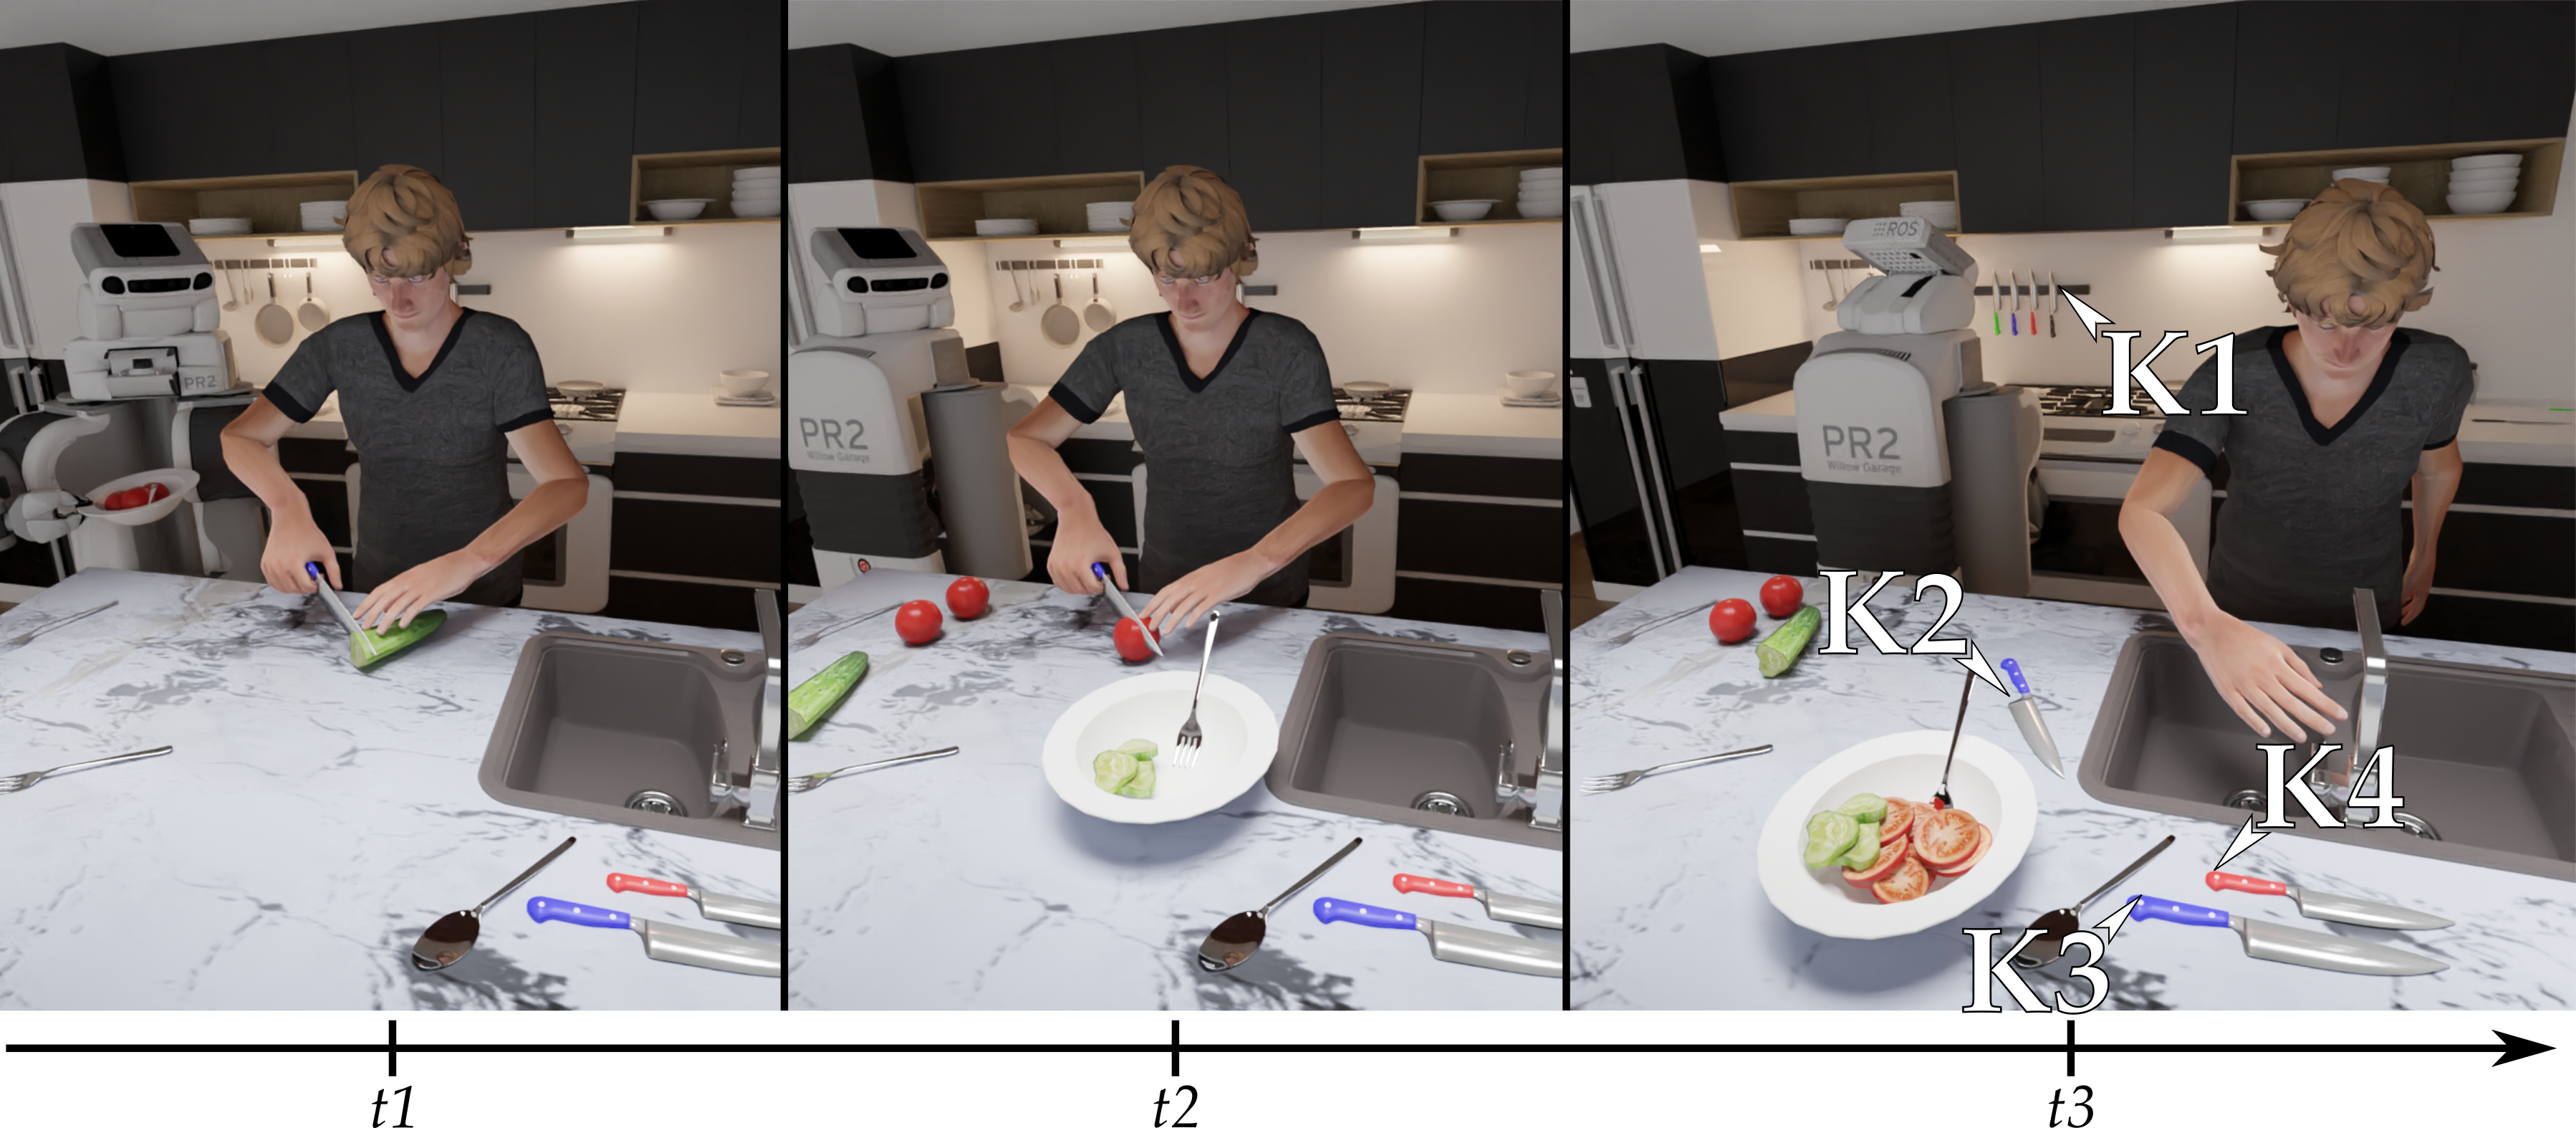
\includegraphics[width=\textwidth]{figures/chapter5/intro/intro.png}
\caption{\label{fig:chap5_intro} A Human-Robot collaborative task with three colored areas and three RFID tags (situation a). The robot has to explain to its human partner to put the tag \textit{o1} in the black area and the tag \textit{o2} in the white area, to reach the situation d. The objects identifiers' are only known to the robot.
If all the communications of the task are not planned ahead, a deadlocked situation could appear if the robot first asks to move the tag \textit{o1} before \textit{o2} (situation b).}
\end{figure}

To better understand the advantage to consider the communication at task planning level, consider the situations of Figure~\ref{fig:chap5_intro}. The robot has to arrange RFID tags on three areas on a table. The robot can identify them with their unique id but being too small, it can not grasp them. On the contrary, the human partner can not identify them uniquely but can grasp them. For this example, we also assume that the robot cannot point to the tags. The robot must therefore communicate the successive actions that the human will have to perform to go from the inial configuration (\ref{fig:chap5_intro} a) to the goal configuration (\ref{fig:chap5_intro} d). Between both configurations, only the tags \textit{o1} and \textit{o2} have to be moved. The tag \textit{o1} has to be moved from the red area to the black and \textit{o2} from the black area to the white. While the tag \textit{o3} can be referred to unambiguously thanks to its color, the two others can not. However, they can be referred thanks to the area they are in (e.g. \textit{``the tag is the red area''}).

If the content of the communications is only refined at execution, two equivalent solutions can be planned (\ref{fig:chap5_intro} sequence a-b-d and a-c-d). At execution, the first solution begins by asking the human to move \textit{o1} in the black area resulting in the instruction \textit{``take the tag that is in the red area and put it in the black area''}. In this new situation where both red tags are now in the black area (Figure~\ref{fig:chap5_intro}b). The robot has no way to designate the tag \textit{o2} without ambiguity. Hence, the task is blocked\footnote{The robot could use spatial relation like right, left, or the closest to me. However, the generation of such \acrshort{re} is not an easy job and the understanding of it neither. Even if the situation is not really blocked, the required communication can be complex. }. Estimating the communication feasibility and cost during the planning process would result in the second possible solution. The robot first ask to move the tag \textit{o2} (Figure~\ref{fig:chap5_intro} c) and then the tag \textit{o1} (Figure~\ref{fig:chap5_intro} d). If the robot could have pointed, the deadlock of the first solution can be avoided with a pointing action and nevertheless, thanks to the communication cost estimation, the least expensive solution can be selected\footnote{Plenty of other solutions could exist but depend on the robot capability. Giving the two instructions in the initial state before the human act solve also the problem for example. Nevertheless, if the robot cannot compare these different solutions regarding its current capability, non-desirable situations could still appear.}.

The main contribution presented in this chapter is an approach to \textbf{estimate the communication feasibility and cost at task planning level}. It implies a fine \textbf{link between a planner and an ontology} to estimate communication grounding in the future estimated state of the environment.

First, we briefly review the literature concerning the task planning problem and discuss the issues we aim to tackle. Then we, give an overview of the involved components with a focus on the task planner while the others have been detailed in the previous chapters. We then present how the fine integration of the components allows us to take estimation the communication at task planning and discuss possible improvement. We end this chapter with three case studies, to show how this approach can be used to prevent deadlocked situations at execution, how it can reduce the global communication complexity during a Human-Robot collaborative task and how it can be used to balance between different communication means.

\section[Related work]{Related work: The need to plan communication}

A significant amount of research has been dedicated to Human-Robot verbal communication, especially to answer the questions of \textit{what} and \textit{when} to communicate~\cite{mavridis_2015_review}. A lot of early works address these questions at execution time, with a fixed plan in which the robot inserts verbal communication afterwards when needed. The communication can be used to share and negotiate plans~\cite{sebastiani_2017_dealing}, to ask for or give specific information~\cite{shah_2011_improved}, to repare errors~\cite{tellex_2014_asking}, align knowledge~\cite{devin_2016_implemented}, or increase trust~\cite{schaefer_2017_communicating}

In the work~\cite{devin_2016_implemented} the robot is provided with a shared plan for both itself and its human partner. On top of that, they use a theory-of-mind enabled framework to estimate, throughout the interaction, the partner's mental state about the current state of the environment and the performed actions. When the robot performs an action while its partner performs another one in a different room, the robot can detect a belief divergence due to the fact that the partner can not know if the robot has acted or not\footnote{This is the case when the action performed by the robot has no observable effects on the environment like scanning object.}. When such divergence is detected, if it can endanger the overall plan, leading the human to perform a wrong action, or block the interaction, verbal communication can be inserted at execution time. It goes the same if the human wait for an action already performed by the robot. The content of the communication is determined with regard to the divergences that can break the shared task.

However, in most cases, deciding communication at execution time is not enough and more recent works deal with communication actions at the planning level. Nikolaidis et al.~\cite{nikolaidis_2018_planning} identify two types of communication: \textit{commands}, where the robot ask for an action to be performed by its partner and \textit{state-conveying} to inform about its internal state. They use a Mixed Observability Markov Decision Processes (MOMDP) to determine the need for communication and its type, returning a policy capturing the probability of the human to take a given action based on the performed communication. A comparable approach is presented by Roncone et al.~\cite{roncone_2017_transparent} with three types of verbal communication action: \textit{command} to provide instruction to the human to perform an action, \textit{ask} to be informed if the human current action is over, and \textit{inform} to communicate an intent. These communications are integrated with others actions into a Partially Observable Markov Decision Process (POMDP) which returns a policy integrating communication actions. However, for both presented approaches, the communication complexity and thus costs are not taken into account. Moreover, while for the first the content is pre-generated, for the second it is not specified at the planning level. This can cause non-achievable communication in some situations.

A similar approach is proposed by Unhelkar et al. \cite{unhelkar_2020_decision} with more communication types considered: \textit{command}, \textit{ask}, \textit{inform} and \textit{answer}. This time, a communication cost is explicitly considered. However, the cost is related to the \textit{when} to communicate and not on the \textit{what}. It is represented by a function penalizing temporally close communication actions. Concerning the content, it is patterns including parameters replaced at execution time. For example, in the sentence \textit{“Please make the next sandwich at -landmark-.”} the sentence representing landmark will be resolved at execution. In their examples, every landmark is assumed to be easily referred to the human, but this is not always the case. Using the \acrshort{reg} at task planning, our approach addresses two of the five challenges identified by Unhelkar et al.: ``estimating benefit of communication'' and ``quantifying cost of communication''~\cite{unhelkar_2017_challenges}.

\begin{figure}[!ht]
\centering
\includegraphics[scale=0.25]{figures/chapter5/tellex.png}
\caption{\label{fig:chap5_tellex} Illustration from \cite{tellex_2014_asking}.
A robot engaged in assembling a table requests help using natural language with targeted requests such as “Please hand me the white table leg." }
\end{figure}

To better understand the difference of our approach regarding existing works, we use the example depicted by Tellex et al. \cite{tellex_2014_asking} and illustrated in Figure~\ref{fig:chap5_tellex}. In this situation, robots, following a precomputed plan, are assembling furniture. During the task, the robot assembling the white table encounter a failure because it can not reach the needed table leg (on the other white table). When such a failure occurs, the robot asks a human for help by referring to the object at the origin of the failure. By doing so, the robot performs a plan reparation with the help of the human and thanks to an object referring communication action. However, if the leg has not been move since the beginning of the task, the non-reachability of the leg could have been known by the robot during the planning process. The non-reachability is not really of failure and such reparation could be avoided. Considering the task as a shared task, the assembly of the leg could be assigned to the human. Keeping the human in the role of a helper, verbal communication still could be planned either to group multiple communications reducing the human disturbance, or to perform it in order to make the communication easier. The robot would have assembly the other white leg to only refer to the last one as ``the white leg'' not leading to any ambiguity with the other ones.


\section{The involved components}

The type of communication actions we want to manage in this chapter is commands using \acrlong{re} presented in the previous chapter. Typical commands will be composed of a static part and a situation-dependent one like \textit{``Take X''}, \textit{``Put it in Y''}, or \textit{``Take X and put it in Y''}. The variable part depends on the state of the situation when the communication is performed and must be solved by a \acrshort{reg}. The communication feasibility and cost thus depend on this variable part and by extension of the moment where it is used.

As explained previously, the \acrshort{reg} aims to be run on the human partner estimated knowledge base to ensure that all the concepts and relations used in the generated \acrshort{re} are known to him. To be able to estimate communication about the future states of the environment and keeping this principle to run on the estimated \acrshort{kb}, we need a symbolic task planner already suitable for \acrshort{hri}. It has to able to distinguish between the different agents involved in the task and to maintain an independent representation of the environment for each of them.

To resolve a specific task, a planner does not necessarily need to be aware of all the elements present in the current environment. It simply needs a representation of the entity that can be used to solve the task. To solve the task of assembling a table, it only needs the table elements for this particular one even if others are present in the environment. Even if we could represent all the elements, it would be counterproductive by not helping to solve the task but adding exploration complexity.
In the same way, it does not need a fine representation of these elements. Even if the task is to create a cube tower with alternating colors, the color information is not necessarily useful. In the introduction example (Figure~\ref{fig:chap5_intro}) the color of the RFID tags does not matter for the task and the type of the objects are also useless. Representing them as movable objects\footnote{To not move the areas around the tags instead of moving the tags.} could be sufficient. Moreover, doing so makes the planner more generic as not being restricted to arrange RFID tags. However, we saw that for the \acrshort{reg}, the more the situation will be described precisely (both in term of types and relation), the more accurate the solution will be. Furthermore, if another tag, which is not part of the task and thus not part of the planner internal representation, is present on the table, it will also impact the \acrshort{reg} and thus the complexity and feasibility of the communication action. 

This difference of representation requirement between the task planner and the \acrshort{reg} lead to the fact that the \acrshort{reg} can not be performed on the planner internal representation. To solve this issue, we have to endow the planner with the ability to maintain a semantic \acrshort{kb} that is used by the \acrshort{reg}. Before going further in the way to solve this challenge, we will first present the newly introduced component as a task planner. We then give more detail about the knowledge base we will consider for this application.


\subsection{The Hierarchical Task Planner}

To implement our approach, we just see that we need a task planner able to maintain an independent estimated knowledge base for each agent involved in the task. We chose the \acrfull{hatp}\footnote{Also called Human-Aware Task Planner}~\cite{lallement_2014_hatp}. \acrshort{hatp} extends the classical \acrfull{htn} planning by being able to produce \textbf{shared plans} to reach a joint goal. A \acrshort{hatp} planning domain describes how to decompose tasks into subtasks down to atomic symbolic actions. Both the robot and human feasible tasks and actions are described in the domain. A context-dependent cost function is associated with each action. 

During the task decomposition, \acrshort{hatp} will explore several applicable sub-tasks until the global task is totally refined into feasible actions, and will return the minimal cost plan. \acrshort{hatp} also supports \textit{social rules}, allowing to balance the effort of involved agents depending on human preferences and to penalize plans presenting certain undesirable sequences of actions. We will not use these social rules in what follows, but our approach stays compatible with them.

Moreover, during the exploration of the task tree, \acrshort{hatp} will assign actions to available agents, robot or human (when an action can be done by both). By doing so, \acrshort{hatp} can elaborate one \textbf{action stream} per agent, together with causality and synchronization links. 
Besides, \acrshort{hatp} domain syntax supports Multiple Values State Variables (MVSV)~\cite{guitton_2012_belief} which is used to represent and reason about each agent mental state. In this way, a given variable can have dfifferent value depending on the represented agent. This allows to represent action preconditions depending on the knowledge of the agent performing the action and also to represent their effect on each agent mental state which can depend on the agent perspective.

Finally, the last argument which motivated our choice was the use of \acrshort{hatp} in previous work: the Geometrical Task Planning (GTP) \cite{gharbi_2015_combining}. This work aimed at refining into motion planning requests the symbolic motion actions explored by \acrshort{hatp} during the task planning process. The motion planner would then returns the feasibility and the cost of the action, but was also able to inform \acrshort{hatp} about why the motion action would not be possible (e.g. the object with which collision would occur). The task planner would then, backtrack to choose a different action to remove the colliding object. This method also shows how to update the geometrically planned environment to match the symbolic one to run the motion planning phase. This approach also needs to update the geometrical planned world to match the symbolic planned knowledge base before running the motion planning phase. This work greatly inspired us, and our approach is similar at the difference that we run a \acrshort{reg} when a communication action is explored, instead of a motion planning request on a symbolic motion task exploration.

\subsection{The semantic knowledge base}

In the previous applications of this thesis, we could use only one knowledge base representing both the robot's and human's knowledge about the environment. This time, because the task planner explicitly manages an independent world state for each agent, we will fully take advantage of Ontologenius to manage several ontology instances at the time. We will thus note the robot's semantic knowledge base $\kbs^R$ and, considering only one partner, the human estimated knowledge base $\kbs^H$. Both will be kept up to date at the same frequence. This means that both represent the knowledge of each agent at the current time. However, as explained in the introduction of this section, we need to run the \acrshort{reg} on a knowledge base that will represent what the robot believes that its partner will know about the future states of the environment. Let us consider the initial state of the introduction example of Figure~\ref{fig:chap5_intro}. The robot plans to remove the tag \textit{o1} from the table and wants to estimate the feasibility of referring the tag \textit{o2} once the first action performed. It thus has to remove \textit{o1} from the table in the estimated knowledge base of the human to evaluate this future communication. Nevertheless, it can not modify $\kbs^H$ as it represents the current estimated knowledge of its partner. Performing such modification could have side effects on the entire robotic architecture. To deal with that we will use the Ontologenius feature that consists of the copy of an existing ontology instance. As a reminder, a copied instance then become independent from the original ontology. The instances representing a future possible mental state of a human will be noted $\kbs^{H_i}$. In this way, the \acrshort{reg} can run on a $\kbs^{H_i}$ for the planning process and on $\kbs^H$ at execution.

\section[Integrating planners]{Integrating task and communication planners}

The general scheme of our approach to enable a symbolic task planner to estimate the feasibility and cost of future communication is the one presented in Figure~\ref{fig:chap5_integration}. On the top of the figure, we have large, complete semantic knowledge bases representing the robot knowledge and the other agents estimated knowledge. At the bottom of the figure, we have the planning process with reduced knowledge bases dedicated to task planning. As explained earlier, because the planning process will need to represent the future estimate mental state of its partner without altering the original estimation, we first perform a copy of the human estimated ontology. From there, it becomes an independent knowledge base, capturing the human knowledge about the environment at a given instant. We call this new ontology the human planned ontology and denote it $\kbs^{H_0}$. At the initialization of the planning process, once the copy is performed, the planner extract from the robot ontology and the human planned ontology the symbolic facts it needs. To do so, every entity types declared in the planning domain are retrieved from the ontologies by their name, and entities inheriting from these types in the ontologies are created in the planning knowledge base. Then, each attribute (both static and dynamic) of every entities declared in the domain has its value updated. If the attribute is a set, multiple relations with the same name originating from the same entity and pointing to different ones can be found in the ontologies. If so, all the pointed entities are added to the set.

\begin{figure}[!ht]
\centering
\includegraphics[scale=0.4]{figures/chapter5/integration.png}
\caption{\label{fig:chap5_integration} A representation of the planning process with the estimation of future human mental states to perform \acrshort{reg}. The ontology representing estimated human knowledge is first copied to plan it without altering the original one. The human and robot planning symbolic facts are extracted from their respective ontologies. During the \acrshort{htn} decomposition, for each verbal communication action encounter, the planned human ontology is updated with the current explored state and the \acrshort{reg} is executed on it. }
\end{figure}

During the task network decomposition, the general workflow executed for each communication action encountered consists of 1) updating the human planned ontology with the expected world state 2) identifying the objects involved in the communication 3) executing the \acrshort{reg} for each of these objects 4) calculating the feasibility and the cost of the communication action according to the feasibility and the cost of each individual \acrshort{re} involved in the planned communication. Note that if multiple objects have to be referred to in single communication (e.g. \textit{``give me X and Y''}), the human planned ontology is only updated once as the estimated state in the same for both \acrshort{reg}.

In this section, we explain how a communication action is represented in the \acrshort{htn} and how the task planner can easily update the human planned ontology. We will even go further with an unimplemented update solution that could reduce the number of updates to be performed. 


\subsection{The representation of the communication action}

To focus ourselves on communication actions, we have thus designed simple planning problems where only the robot knows the goal of a joint task and issues command to its human partner one at a time when the human has to do an action. Communications related to entities of the scene are thus needed in each step of the plan because the human has no way to guess the actions he has to perform. Even if these problems present major limitations regarding the \textit{when} to communicate it allows us to simply present our approach. However, the method is still applicable on more general problems which need to estimate the \textit{what} of communications and ensure their pertinence in future states. Moreover, the presented method is compatible with others, focused on the estimation of the \textit{when} to communicate~\cite{devin_2016_implemented}, \cite{unhelkar_2020_decision}.

In the \acrshort{hatp} domain it is represented in the way that when an abstract or a primitive task is only feasible by a human and requires to designate a specific entity, a decomposition is added. In this decomposition, we specify that if the task is assigned to a human, a referring communication action must be done before by the robot in the direction of this human. This kind of decomposition is needed because we place ourselves in cases where the human partner does not know the global objectives of the task, and thus, all the instructions must be given by the robot. With this approach, we consider that the human needs communication from the robot to act, and does not plan by himself. In a more general case, the communication action from the robot would only appear if humans do not have the necessary information~\cite{devin_2016_implemented}. An example of plan is represented in Figure~\ref{fig:chap5_plan}.

\begin{figure}[!ht]
\centering
\includegraphics[width=\textwidth]{figures/chapter5/plan.png}
\caption{\label{fig:chap5_plan} An example of a plan generated by \acrshort{hatp} where the robot instructs to take an object then place it in an area. Green actions are performed by the human while the bicolor actions involve both agents. }
\end{figure}

The communication action feasibility is then determined by both symbolic preconditions (e.g. the human and the robot are in the same room) and \acrshort{reg} result (whether a solution is found or not). If the communication action is feasible, the cost of the communication action is then computed as the sum of a fixed cost depending on the type of communication and the \acrshort{reg} solution cost. If multiple entities would have to be referred in a single communication, the cost would be the sum of each \acrshort{reg} solution cost and the fixed cost.

\subsection{Maintaining the right knowledge base, at the right time}

We previously saw the need to keep an ontology updated with the estimated beliefs at the time of the communication to run the \acrshort{reg} on it and the necessity to create the human planned ontology with a copy of the human estimated one to not create side effect on the rest of the architecture.

Since maintaining this external representation can be a heavy process, we first choose to only update it when a communication action has to be evaluated. However, having a single planned ontology, knowing the update to perform on it to reflect the current explored state can be an intractable problem. The planner could perform backtracking during the exploration in order to determine the modifications to perform to represent the state of the currently evaluated communication. Consequently, the modifications would depend on the previous communication action explored. Because the previous communication could come from a side decomposition, the planner would have to either compare each relation between its representation and the ontology or keep a trace of all the modifications between two successive evaluations.

A first solution would be to create a copy of the planned ontology representing the initial state in order to have one ontology for each communication evaluation, all created from the initial state. Such a solution would reduce the planner complexity but as the ontology represents a superset of the planner facts base, it would be too time-consuming for the ontologies manager. For huge ontologies, analyzing the modification between two updates would be faster than an entire copy.

To solve this problem we thus choose to use a versioning system on the ontology. This versioning system is the one proposed by the software Ontologenius presented in Chapter~\ref{chap:2}\footnote{For the story of this thesis, this functionality was initially developed especially for this application.}. We thus keep the first step that is to create the planned ontology with a copy then perform a commit on it to mark this initial state. From there, when a communication action is found, the planner goes back to the initial commit and update the ontology with the difference from the initial state. However, \acrshort{hatp} is not adapted to keep such trace and it would require too many modifications in its internal structure. To pass over this problem, the planner performs a first commit to represent the initial state and extract the necessary knowledge from it. It then removes all the dynamic relations from the ontology and performs a second commit. It will represent a kind of pattern for each state involving a communication action. For each of them, the planner just has to go back to the commit representing this pattern and update all the dynamic relations with their values in the evaluated state. An example of a commit-graph related to this solution is represented in Figure~\ref{fig:chap5_versioning_simple}. Each commit thus represents a $\kbs^{H_i}$ on which a \acrshort{reg} can be performed. The advantage here is that the knowledge backtracking is internally managed by Ontologenius and thus optimized.

\begin{figure}[!ht]
\centering
\includegraphics[scale=0.3]{figures/chapter5/versioning_simple.png}
\caption{\label{fig:chap5_versioning_simple} The commit-graph generated by Ontologenius for a plan with three communication action evaluated. Each evaluation generates a specific commit representing the state of the world at the moment of the communication. }
\end{figure}

\subsection{Reducing the number of updates}

A major limitation of the previous solutions is the need to update all the dynamic relations even if few changes have been made between communications. An unimplemented but feasible solution would be to update the ontology for each explored state during the planning process and create a commit for each of them. The advantage is that the backtracking has not to be managed by the task planner and only the modified relations have to be updated in the ontology. A commit-graph of such solution is represented in Figure~\ref{fig:chap5_versioning_advance}. Assuming this graph to represent the same task decomposition of the previous one, we see however that more commits have to be performed even if fewer modifications are performed between the two. For tasks with many communication actions, it could lead to a performance gain but for tasks with less communication, it would require more updates than needed as even decompositions without communication have to update the ontology.

\begin{figure}[!ht]
\centering
\includegraphics[scale=0.25]{figures/chapter5/versioning_advance.png}
\caption{\label{fig:chap5_versioning_advance} The commit-graph generated by Ontologenius for a plan with three communication action evaluated. Each explored state, with ou without communication action, generates a specific commit representing the state of the world at the moment of the action. }
\end{figure}

From the planner point of view, it would just have to assign UID to each state and created a commit using these UIDs. When backtracking, it would just have to checkout the ontology with the UID of the state to explore.

\newpage

\section{Results}

In this section, we present three case studies. The two first ones are run in simulation with only minimalist setups. They respectively show that the estimation of the communication content during the task planning 1) can prevent from execution dead-end and 2) can reduce the global communication complexity during the task. The third case study is run on a PR2 robot. It shows that our method makes it possible to compare different means of communication and to choose the most appropriate. The integration in the robotic architecture is presented in the next section.

All the three cases studies are based on a cube arrangement task in the same principle of the RFID tag arrangement presented in introduction. The human can only distinguish the cubes by their color and the digit written on them (one or two) if there is one. Three colored storage areas cover the entire surface of the table. An object is thus always in one of the areas. The area in which the cube is, is an additional information usable for the communication. The most complete \acrshort{re} is of the kind of: \textit{``the green cube with the number 2 which is in the black area''}. For the three cases, only the robot knows the goal configuration but can not manipulate the cubes. It thus has to guide the human in the arrangement task. The robot can only point the cubes in the third case study. In the first two, it can only use verbal communication.

\subsection{Prevent execution dead-end}

In this first case study, we consider the introduction example recall in Figure~\ref{fig:chap5_case1} with the initial state (left) and final state (right). The cube C1 has to be moved from the red area to the black area. The cube C2 has to be moved from the black area to the white area. The cube C3 does not have to be moved.

\begin{figure}[!ht]
\centering
\includegraphics[width=\textwidth]{figures/chapter5/results_case1.png}
\caption{\label{fig:chap5_case1} The initial state (left) and final state (right) of a task where the robot has to explain to the human partner how to move the cubes to complete the task. In this situation, explaining C2 first then C1 avoids a dead-end. }
\end{figure}

Taking into account the cost and the feasibility of the communication, we found with our method the plan of Listing~\ref{lst:chap5_case1}. Cube C2 is moved first then the cube C1. Doing the inverse order, after moving C1, the two cubes would be in the black area at the same time. Such a situation would cause a dead-end during the execution of the plan or at least require complex communication. Actions prefixed with HR are performed simultaneously by the robot and the human while the actions prefixed by H are only performed by the human. As a comment of each action are the relations to communicate.

\begin{lstlisting}[frame=single, basicstyle=\scriptsize\ttfamily, label={lst:chap5_case1}, caption={The obtained plan for the first case study where cube C1 must be moved from the red to the black area and cube C2 moved from the black to the white area. The lines beginning with H represent the actions of the human and the lines beginning with HR represent actions involving the human and the robot (communication actions). In green are the \acrshort{reg} results for each communication action.}, captionpos=b, style=HatpPlan]
HR - TellHumanToTake(C2) // (C2, isA, Cube), (C2, isIn, area_black), 
                         // (area_black, isA, Area), 
                         // (area_black, hasColor, black)
H  - Take(C2)
HR - TellHumanToPlace(C2, area_white) // (area_white, isA, Area),
                                      // (area_white, hasColor, white)
H  - Place(C2, area_white)
HR - TellHumanToTake(C1) // (C1, isA, Cube), (C1, isIn, area_red), 
                         // (area_red, isA, Area), (area_red, hasColor, red)
H  - Take(C1)
HR - TellHumanToPlace(C1, area_black)  // (area_black, isA, Area),
                                       // (area_black, hasColor, black)
H  - Place(C1, area_black)
\end{lstlisting}

Considering once again the same initial state but with the goal to invert the positions of the two cubes, if the communication cost and feasibility are not taken into account during planning, both actions directly leading to the goal state (\textit{i.e.} cube C1 moved to the black area or cube C2 to the red area) will lead to a dead-end at plan execution. To solve this situation, the task planner chooses to add a supplementary action. It consists of putting the cube C1 in the white area that then leads to a problem similar to the previous one. This additional action avoids a dead-end by making communication about cube C2 feasible. Another solution could have been to move C2 in the white area first, leading once again to a situation comparable to the previous one.

\subsection{Reduce the overall communication complexity}

\begin{figure}[!ht]
\centering
\includegraphics[width=\textwidth]{figures/chapter5/results_case2.png}
\caption{\label{fig:chap5_case2} The initial state (left) and final state (right) of a task where the robot has to explain to the human partner how to move the cubes to complete the task. In this situation, explaining C2 first then C3 is easier than the inverse. }
\end{figure}

In this second case study, we show how the estimation of communication can be used to reduce the complexity of global communication. We consider the initial state and the goal state represented in Figure~\ref{fig:chap5_case2}. Only cubes C2 and C3 should be moved. Our method finds the solution consisting of moving cube C2 first, then cube C3. With this order, cube C2 is referred by three relations: its type (\textit{i.e.} cube), the number on it, and the colored area in which it is located. After that, the cube C3 can also be referred to using only three relations being its type, its color and the colored area in which it is located. Considering the reverse order, this would have generated a more complex \acrshort{re} first for cube C3 with four relations: its type, its color, the number on it and the colored area in which it is located.
The solution chosen by our method communicates a sum of six relations rather than seven with the reverse order.

\subsection{Compare with other communication means}

In this last case study, we show how the estimation of verbal designation communication cost can be used to compare it with other communication means, here pointing. Now, we consider twelve cubes. The initial state and the goal state are represented in Figure~\ref{fig:chap5_case3}. Such a number of similar objects leads to long explanations to refer to certain cubes. Therefore, we aim the task planner to choose another means of communication to refer to cubes too difficult to explain verbally. The pointing action has a constant cost which is higher than simple verbal communication but lower than a complex one (with three or more relations to verbalize). To exemplify the comparison with other communication means, the arrangement order is predefined in this setup.

\begin{figure}[!ht]
\centering
\includegraphics[width=\textwidth]{figures/chapter5/results_case3.png}
\caption{\label{fig:chap5_case3} The initial state (left) and final state (right) of a task where the robot has to explain to the human partner how to move the cubes to complete the task. In this situation, some cubes are too complex to explain. Pointing them could help in some cases. }
\end{figure}
 
The generated plan is available in appendix~\ref{app:reg_com_plan}. The cubes C5 and C7 are chosen to be pointed instead of verbalized. Indeed, in the world states where these cubes need to be moved, verbal referring is considered to be too costly, thus a pointing motion is preferred. For example, the cube C5 in the initial situation needs a long and complex explanation that is: \textit{``take the black cube with the number two which is in the black area''}. Even in the cases where the pointing action takes more execution time, it could require less cognitive load for the human partner and so make the human action faster.

Here, we see another benefit of our approach, it allows the planner to balance between the use of verbal communication actions, which can become complex in some states (hard to predict without a task planner), and other communication modalities. Here, balancing was done with other means of communication, but it could also be done with other actions such as a pick and place by the robot. In the task presented here, this has no advantage, because a pick and place by the robot would be slower than an explanation or a pointing and is more likely to fail.

\section{Integration in a robotic system}

The third case study has been implemented and integrated on a pr2 robotic platform. We extend the previously used architecture and integrate two new components as illustrated in Figure~\ref{fig:chap5_archi}. The execution of the third case can be found in the video available at \url{https://youtu.be/3YnGh_t-UpY}.

\begin{figure}[!ht]
\centering
\includegraphics[scale=0.6]{figures/chapter5/architecture.png}
\caption{\label{fig:chap5_archi} The architecture used to validate the method. The knowledge bases are continuously kept up to date through the situation assessment. The task planner can query the \acrshort{reg} to estimate the feasibility and cost of future communications. }
\end{figure}

The Symbolic task planner is \acrshort{hatp}. It is requested by the supervision component which is able to manage the execution of the generated shared plan. The task planner can recover the initial state from the semantic knowledge base and update an ontology instance to represent the human future estimated knowledge base. In addition, it can request the generation of referring expression on a human planned ontology.

The second newly integrated component is a motion planner and execution component. For now, it only provides to the supervision a pointing service and automatically chooses the arm to point with. However, it does not consider the obstacles.

The geometrical situation assessment component has been changed from Robosherlock to a custom version of Toaster\footnote{https://github.com/sarthou/toaster}. It is the successor of the software SPARK~\cite{milliez_2014_framework}. It can take as inputs several perception modalities and merge them in a coherent geometric representation. For our implementation, we simply use AR-tags which give precise enough position and allow us to identify objects with UIDs. The table and other static elements of the environment are not perceived and provided as static elements. The three storage areas are neither perceived and described as 3D virtual areas. Thanks to these areas, Toaster is able to compute the fact \textit{isIn} for each of the cubes. From there, Toaster has been linked to Ontologenius to update the ontologies continuously. A representation of Toaster geometric environment is represented in Figure~\ref{fig:chap5_toaster}.

\begin{figure}[!ht]
\centering
\includegraphics[scale=0.70]{figures/chapter5/toaster.png}
\caption{\label{fig:chap5_toaster} A visual representation in Rviz of the geometric state of the managed by Toaster. While the cubes are perceived with tags, the other elements are static.
 }
\end{figure}

A major limitation of the current situation assessment component is that it can not perform perspective-taking. This means that even if it can represent the human as a particular entity, it can not estimate the state of the world from the human point of view\footnote{We can compute if an object is in the field of view of the human but not working with a graphical engine, it can not take into account the occlusions.}. It is not a problem for our application since all the elements are visible for both agents and the entire interaction is performed around the table. Toaster thus updates the robot and human ontologies with the same facts. \\

With this integration, the robot is thus able to analyse the current situation, and then to generate a plan to choose the more adapted communication mean for each cube to be moved. Consequently, at execution, at each step of the plan, the robot either verbally explains the cube to take or point to it.
